%FOR PDFLATEX USE ONLY
\documentclass[a4paper,12pt]{article}

\usepackage{amssymb,amsmath} %math symbols

\usepackage[margin=2cm]{geometry} %paper geometry

\usepackage[T1, T2A]{fontenc}

\usepackage[utf8]{inputenc} %allows unicode (including russian) source file
\usepackage[russian]{babel} %docment in russian-style
\usepackage[utf8]{inputenc}
%\usepackage[unicode]{hyperref} %links inside of the text
\usepackage[pdftex]{graphicx} %includegraphics pictures
\usepackage{cmlgc} %bold text

\usepackage{array} %arrays

%\usepackage{wrapfig}
%\usepackage{array}
%\usepackage{lipsum}
%\usepackage{esvect}
%\usepackage{hyperref}

\usepackage{amsmath}
\usepackage{amssymb}
\usepackage{mathtools}
\usepackage{mathtext}

\usepackage{subfig}
%\usepackage{calc}
%\usepackage{pgfplots,tikz,circuitikz}
%\usepackage{tkz-euclide}

\begin{document}

\begin{center}
  \LARGE{Работа 3.6.1}\\[0.2cm]
  \LARGE{Спектральный анализ электрических сигналов}\\[0.2cm]
  \large{Стрижак Даниил}\\[0.2cm]
\end{center}  
  

\section{Аннотация}

В работе изучается спектральный состав периодических электрических сигналов различной формы: последовательности прямоугольных импульсов, последовательности цугов и амплитудно модулированных гармонических колебаний. Спектры этих сигналов наблюдаются с помощью промышленного анализатора спектра и сравниваются с рассчитанными теоретически. 

\section{Теоретические сведения}

Сколь угодно сложный электрический сигнал V (t) может быть разложен на более простые сигналы. В радиотехнике широко используется разложение сигнала V (t) на совокупность гармонических сигналов различных частот $\omega$. Функция F($\omega$), описывающая зависимость амплитуд отдельных гармоник от частоты, называется амплитудной спектральной характеристикой сигнала V (t). Представление сложного периодического сигнала в виде суммы дискретных гармонических сигналов в математике называется разложением в ряд Фурье.

Зная спектральный состав F($\omega$) периодической последовательности некоторого импульса V (t), мы можем осуществить обратное преобразование Фурье: сложив отдельные гармоники со своими амплитудами и фазами, получить необходимую последовательность импульсов. Степень совпадения полученного сигнала с V (t) определяется количеством синтезированных гармоник: чем их больше, тем лучше совпадение.

Рассмотрим конкретные примеры периодических функций, которые будут предметом исследования в нашей работе.

\subsection{Спектральный анализ электрических сигналов}

\begin{center}
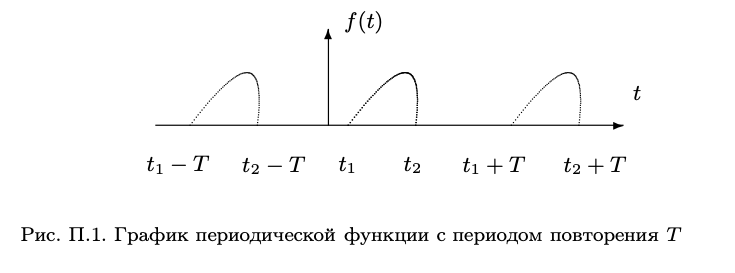
\includegraphics[width=0.7\linewidth]{1.jpg}\\
\end{center}

Пусть заданная функция $f(t)$ периодически повторяется с частотой $\Omega_{1}=2 \pi / T,$ где $T-$ период повторения $($ рис. $\Pi .1) .$ Её разложение в ряд Фурье имеет вид
$$
f(t)=\frac{a_{0}}{2}+\sum_{n=1}^{\infty}\left[a_{n} \cos \left(n \Omega_{1} t\right)+b_{n} \sin \left(n \Omega_{1} t\right)\right]
$$
или
$$
f(t)=\frac{A_{0}}{2}+\sum_{n=1}^{\infty} A_{n} \cos \left(n \Omega_{1} t-\psi_{n}\right)
$$
Здесь $a_{0} / 2=A_{0} / 2-$ постоянная составляюпдая (среднее значение) функции $f(t) ; a_{n}$ и $b_{n}-$ амплитуды косинусных и синусных членов разложе-ния. Они определяются выражениями
$$
\begin{array}{l}
a_{n}=\frac{2}{T} \int_{t_{1}}^{t_{1}+T} f(t) \cos \left(n \Omega_{1} t\right) d t \\
b_{n}=\frac{2}{T} \int_{t_{1}}^{t_{1}+T} f(t) \sin \left(n \Omega_{1} t\right) d t
\end{array}
$$

Точку начала интегрирования $t_1$ можно выбрать произвольно.
В тех случаях, когда сигнал чётен относительно t = 0, в тригонометрической записи остаются только косинусные члены, т.к. все коэффициенты $b_n$ обращаются в нуль. Для нечётной относительно t = 0 функции, наоборот, ряд состоит только из синусных членов.

Амплитуда $A_{n}$ и фаза $\psi_{n} n$ -й гармоники выражаются через $a_{n}$ и $b_{n}$ следуюшим образом:
$$
A_{n}=\sqrt{a_{n}^{2}+b_{n}^{2}} ; \quad \psi_{n}=\operatorname{arctg} \frac{b_{n}}{a_{n}}
$$
Как мы видим, спектр любой периодической функции состоит из набора гармонических колебаний с дискретными частотами: $\Omega_{1}, 2 \Omega_{1}, 3 \Omega_{1}$ $\ldots$ и постоянной составляющей, которую можно рассматривать как колебание с нулевой частотой $\left(0 \cdot \Omega_{1}\right) .$

Представим выражение в комплексной форме. Для этого заменим косинусы экспонентами в соответствии с формулой
$$
\cos \alpha=\frac{e^{i \alpha}+e^{-i \alpha}}{2}
$$
Подстановка даёт
$$
f(t)=\frac{1}{2}\left(A_{0}+\sum_{n=1}^{\infty} A_{n} e^{-i \psi_{n}} e^{i n \Omega_{1} t}+\sum_{n=1}^{\infty} A_{n} e^{i \psi_{n}} e^{-i n \Omega_{1} t}\right)
$$
Введём комплексные амплитуды $\tilde{A}_{n}$ и $\tilde{A}_{-n}$

$$
\tilde{A}_{n}=A_{n} e^{-i \psi_{n}} ; \quad \tilde{A}_{-n}=A_{n} e^{i \psi_{n}} ; \quad \tilde{A}_{0}=A_{0}
$$
Разложение $f(t)$ приобретает вид
$$
f(t)=\frac{1}{2} \sum_{n=-\infty}^{\infty} \tilde{A}_{n} e^{i n \Omega_{1} t}
$$

Как мы видим, введение отрицательных частот (типа −n$\Omega_1$) позволяет записать разложение Фурье особенно простым образом. 

Для расчёта комплексных амплитуд $A_{n}$ yмножим левую и правую части на $e^{-i k \Omega_{1} t}$ и проинтегрируем полученное равенство по времени на отрезке, равном одному периоду, например, от $t_{1}=0$ до $t_{2}=2 \pi / \Omega_{1} .$ В правой части обратятся в нуль все члены, кроме одного, соответствующего $n=k .$ Этот член даёт $A_{k} T / 2 .$ Имеем поэтому
$$
A_{k}=\frac{2}{T} \int_{0}^{T} f(t) e^{-i k \Omega_{1} t} d t
$$
Рассмотрим периодические функции, которые исследуются в нашей paбoтe.


\subsection{Периодическая последовательность прямоугольных импульсов}
C амплитудой $V_{0},$ длительностью $\tau,$ частотой повторения $f_{\text {повт }}=1 / T,$ где $T-$ период повторения импульсов.


Cреднее значение


\langle V\rangle=\frac{a_{0}}{2}=\frac{A_{0}}{2}=\frac{1}{T} \int_{-\tau / 2}^{\tau / 2} V_{0} d t=V_{0} \frac{\tau}{T}

Амплитуды косинусных составляющих равны
$$
a_{n}=\frac{2}{T} \int_{-\tau / 2}^{\tau / 2} V_{0} \cos \left(n \Omega_{1} t\right) d t=2 V_{0} \frac{\tau}{T} \frac{\sin \left(n \Omega_{1} \tau / 2\right)}{n \Omega_{1} \tau / 2} \sim \frac{\sin x}{x}
$$
Поскольку наша функция чётная, все амплитуды синусоидальных гармоник $b_{n}=0 .$ Спектр $F(\nu)$ последовательности прямоугольных импульсов представлен на рис. П.3. Амплитуды гармоник $A_{n}$ меняются по Закону $(\sin x) / x$
На рис. П.3 изображён спектр для случая, когда $T$ кратно $\tau .$ Назовём шириной спектра $\Delta \omega$ (или $\Delta \nu$ ) расстояние от главного максимума $(\nu=0)$ до первого нуля, возникающего, как нетрудно убедиться, при $\Omega_{1}=2 \pi / \tau$ При этом
$$
\Delta \omega \tau \simeq 2 \pi \quad \text { или } \quad \Delta \nu \Delta t \simeq 1
$$
Полученное соотношение взаимной связи интервалов $\Delta \nu$ и $\Delta t$ является
частным случаем соотношения неопределенности в квантовой механике. Несовместимость острой локализации волнового процесса во времени с узким спектром частот - явление широко известное в радиотехнике. Ширина селективной настройки $\Delta \nu$ радиоприёмника ограничивает приём радиосигналов Длительностью $t<1 / \Delta \nu$

 \begin{center}
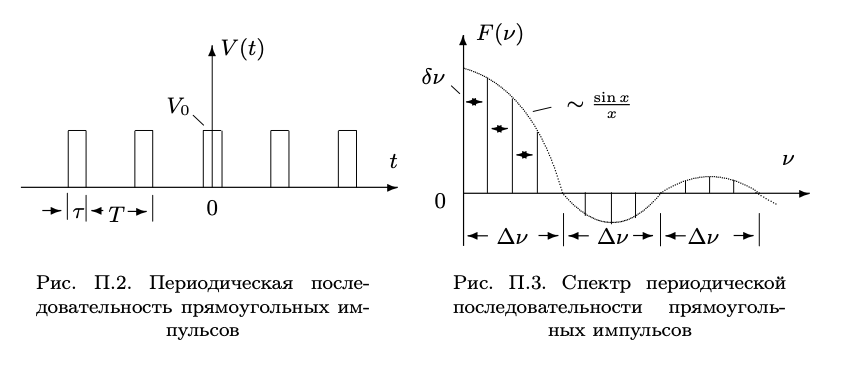
\includegraphics[width=0.7\linewidth]{2.jpg}\\
\end{center}

\subsection{Периодическая последовательность цугов}
Гармонического колебания $V_{0} \cos \left(\omega_{0} t\right)$ с длительностью цуга $\tau$ и периодом повторения $T$ (рис. $\Pi .4)$
 
Функция $f(t)$ снова является чётной относительно $t=0 .$ Амплитуда $n$ -й гармоники равна
$$
\begin{array}{c}
A_{n}=a_{n}=\frac{2}{T} \int_{-\tau / 2}^{\tau / 2} V_{0} \cos \left(\omega_{o} t\right) \cdot \cos \left(n \Omega_{1} t\right) d t= \\
=V_{0} \frac{\tau}{T}\left(\frac{\sin \left[\left(\omega_{0}-n \Omega_{1}\right) \frac{\tau}{2}\right]}{\left(\omega_{0}-n \Omega_{1}\right) \frac{\tau}{2}}+\frac{\sin \left[\left(\omega_{0}+n \Omega_{1}\right) \frac{\tau}{2}\right]}{\left(\omega_{0}+n \Omega_{1}\right) \frac{\tau}{2}}\right)
\end{array}
$$

Такое спектральное распределение F ($\omega$) для случая, когда $\frac T\tau$ равно целому числу, представлено на рис. П.5. Сравнивая спектр последовательности прямоугольных импульсов и спектр цугов (см. рис. П.3 и П.5), мы видим, что они аналогичны, но их максимумы сдвинуты по частоте на величину $\omega_0$.

\begin{center}
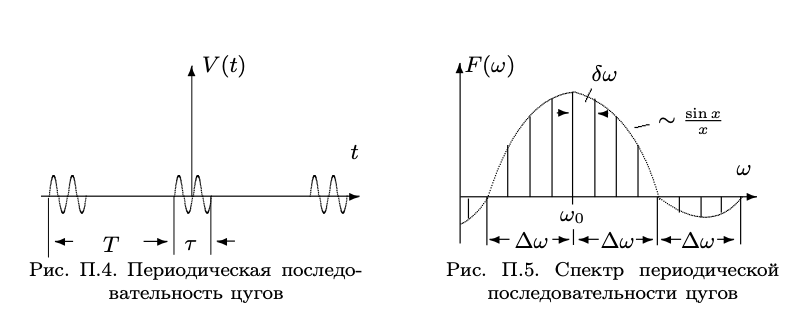
\includegraphics[width=0.7\linewidth]{3.jpg}\\
\end{center}

\subsection{Амплитудно-модулированные колебания.}

\begin{center}
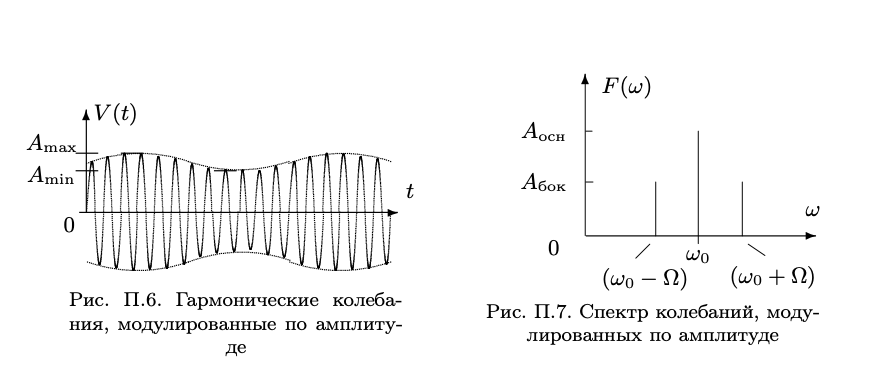
\includegraphics[width=0.7\linewidth]{4.jpg}\\
\end{center}
 Рассмотрим гармонические колебания высокой частоты $\omega_{0},$ амплитуда которых медленно меняется по гармоническому закону с частотой $\Omega\left(\Omega \ll \omega_{0}\right)$ (рис. П.6):
$$
f(t)=A_{0}[1+m \cos (\Omega t)] \cos (\omega t)
$$
Коэффициент $m$ называют глубиной модуляции. При $m<1$ амплитуда колебаний меняется от минимальной $A_{\min }=A_{0}(1-m)$ до максимальной $A_{\max }=A_{0}(1+m) .$ Глубина модулящии может быть представлена в виде
$$
m=\frac{A_{\max }-A_{\min }}{A_{\max }+A_{\min }}
$$
Простым тригонометрическим преобразованием можно найти спектр амплитудно-модулированных колебаний:
$$
\begin{aligned}
f(t) &=A_{0} \cos \left(\omega_{0} t\right)+A_{0} m \cos (\Omega t) \cos \left(\omega_{0} t\right)=\\
=A_{0} \cos \left(\omega_{0} t\right) &+\frac{A_{0} m}{2} \cos \left(\omega_{0}+\Omega\right) t+\frac{A_{0} m}{2} \cos \left(\omega_{0}-\Omega\right) t
\end{aligned}
$$

Спектр $F(\omega)$ таких колебаний содержит три составляюшцих (рис. П. 7$)$ Основная компонента представляет собой исходное немодулированное колебание с иесущей частотой $\omega_{0}$ и амплитудой $A_{\mathrm{ocн}}=A_{0}-$ первое слагаемое в правой части; боковые компоненты спектра соответствуют гармоническим колебаниям с частотами $\left(\omega_{0}+\Omega\right)$ и $\left(\omega_{0}-\Omega\right)-$ Второе и третье слагаемые. Амплитуды этих двух колебаний одинаковы и составляют $m / 2$ от амплитуды немодулированного колебания: $A_{\text {бок }}=A_{0} m / 2$

\newpage

\section{Результаты измерений и обработка данных}

Соберем схему и подготовим приборы к работе, следуя техническому описанию, расположенному на установке.

\subsection{Часть А}

B этой части исследуется зависимость ширины спектра периодической последовательности прямоугольных импульсов от длительности отдельного импульса.

Установим на анализаторе спектра режим работы с однократной развёрткой и получим на экране спектр импульсов с параметрами $f_{\text {повт}}=10^{3}  Гц ; } \tau=100$ мкс; частотный масштаб $m_{x}=5$ к Гц / дел.

Проанализируем, как меняется спектр 

a) при увеличении $\tau$ вдвое при неизменном $f_{\text {повт }}=1$ кГц. $\Delta \nu$ -- уменьшается вдвое, $\delta \nu$ -- остается неизменным. \\

\begin{minipage}{0.44\textwidth}
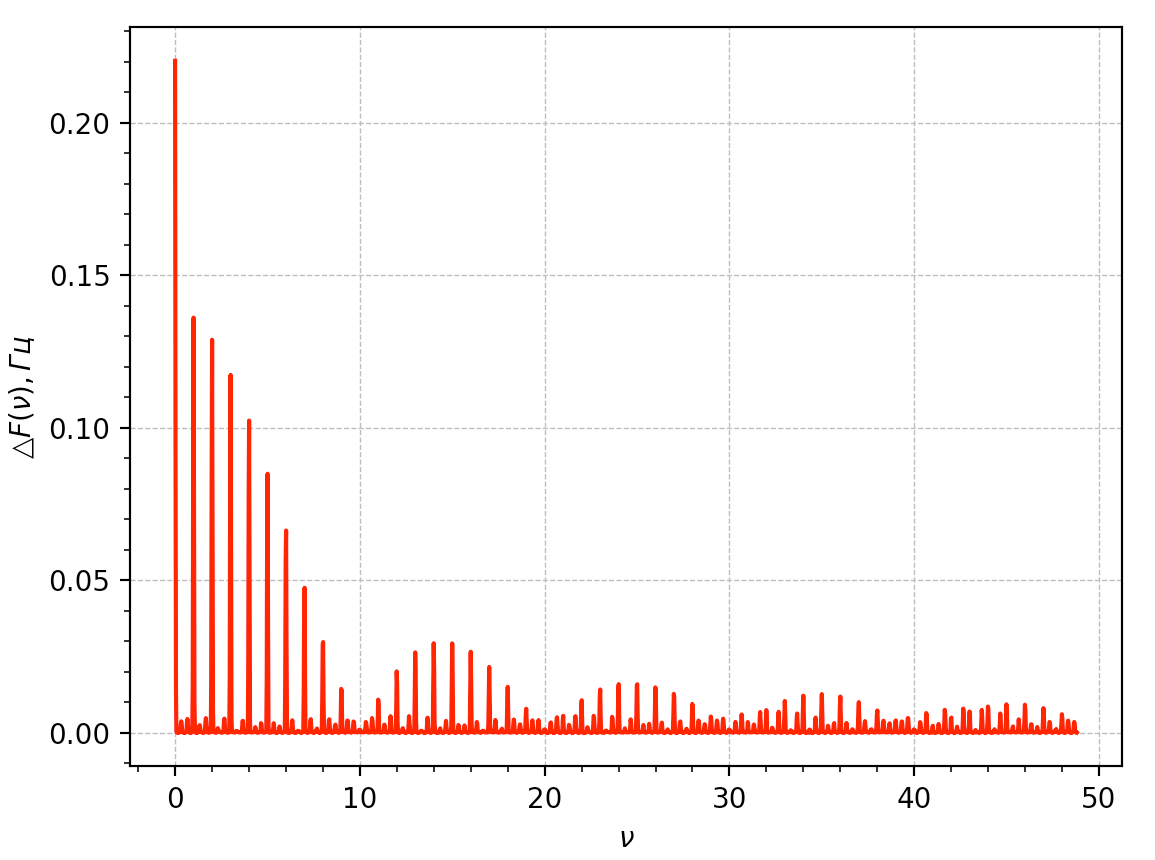
\includegraphics[width=\linewidth]{1.png}\\
\begin{center}
"Эталонный спектр"
\end{center}
\end{minipage}
\begin{minipage}{0.1\textwidth}
\ \ \ \ \ \ \Rightarrow
\end{minipage}
\begin{minipage}{0.44\textwidth}
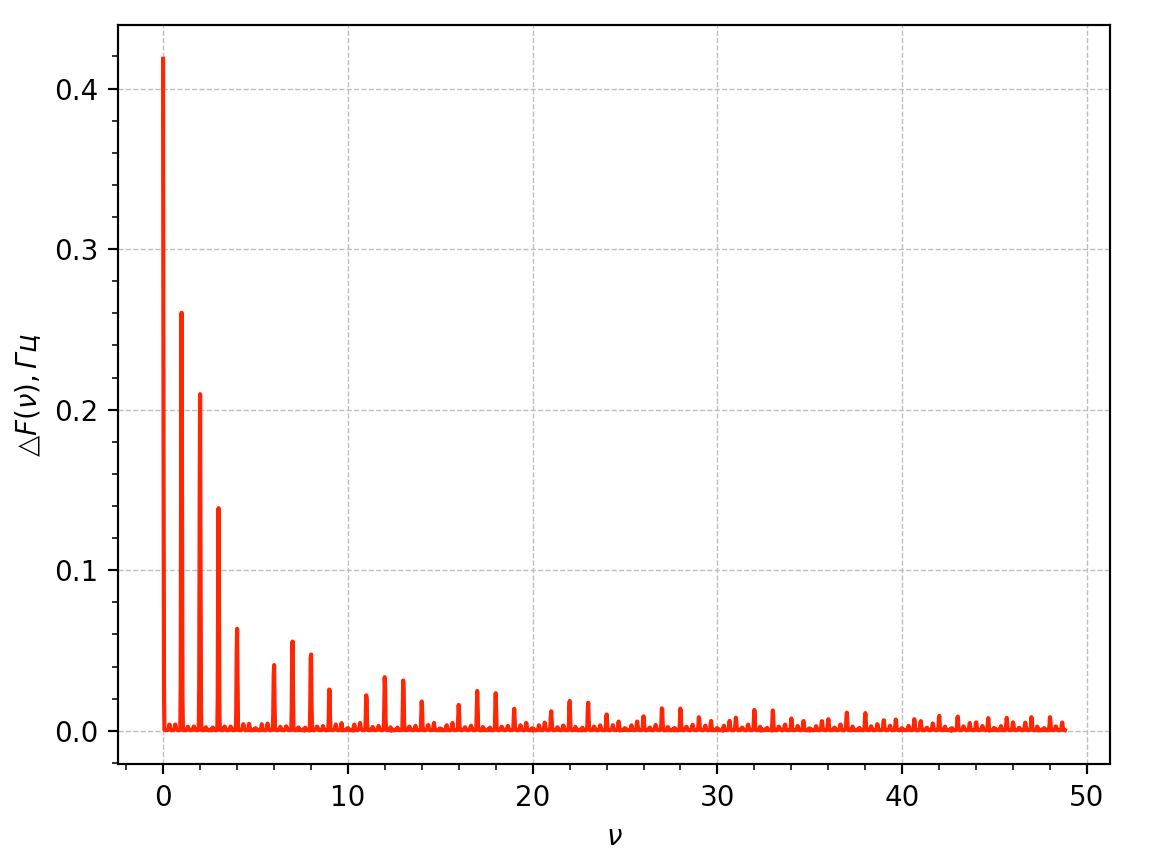
\includegraphics[width=\linewidth]{2.png}\\
\begin{center}
"Увеличение $\tau$ вдвое"
\end{center}
\end{minipage}

\\
\
\\
\

б) при увеличении $f_{\text {повт }}$ вдвое при неизменном $\tau=100$ мкс. $\Delta \nu$ -- остается неизменным, а $\delta \nu$ -- увеличивается вдвое. 

\begin{minipage}{0.44\textwidth}
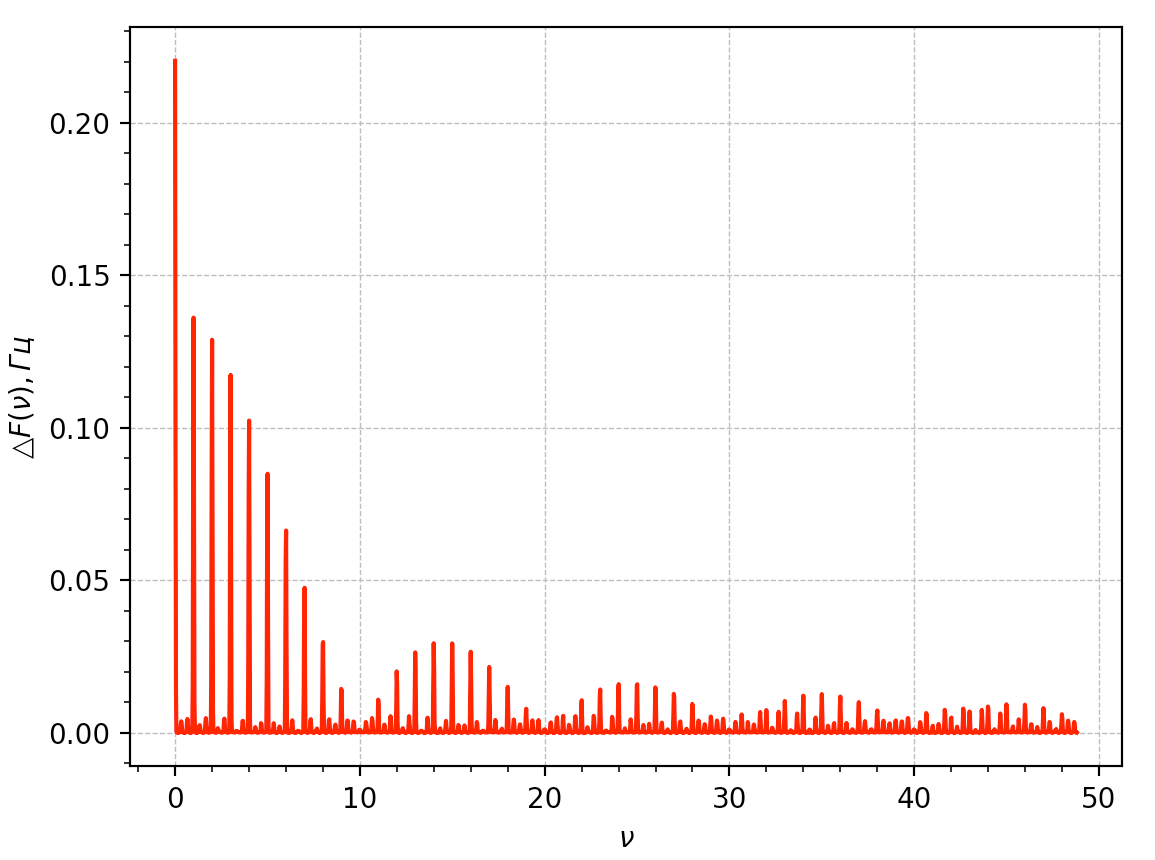
\includegraphics[width=\linewidth]{1.png}\\
\begin{center}
"Эталонный спектр"
\end{center}
\end{minipage}
\begin{minipage}{0.1\textwidth}
\ \ \ \ \ \ \Rightarrow
\end{minipage}
\begin{minipage}{0.44\textwidth}
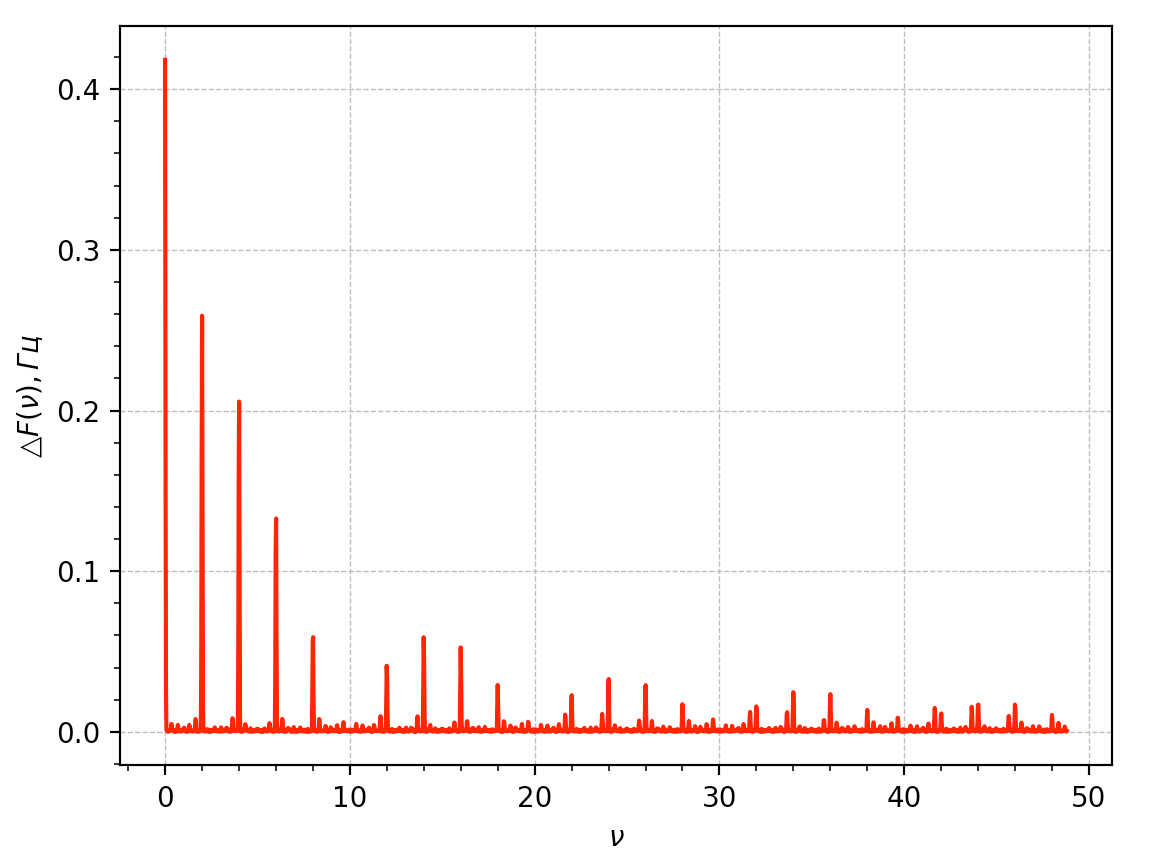
\includegraphics[width=\linewidth]{3.png}\\
\begin{center}
"Увеличение $f_{повт}$ вдвое"
\end{center}
\end{minipage}

\\

\
\newpage
Проведем измерения зависимости ширины спектра от длительности импульса $\Delta \nu(\tau)$ при увеличении $\tau$ от 40 до 200 мкс при $f_{\text {повт }}=1$ кГц.\\

\begin{minipage}{0.3\textwidth}
\begin{tabular}{|c|c|c|c|}
		\hline
		\Delta \nu   & \tau, мкс &$ \frac{1}{\tau}, $мкс^{-1}$ \cdot 10^2 $ \\ 
		\hline
25   & 40&2,50\\ 
		\hline
17     &60&1,67 \\ 
		\hline
13     &  80&1,25 \\ 
		\hline
10     &  100&1,00\\ 
		\hline
 9     & 120&0,83 \\ 
		\hline
7    & 140& 0,71\\ 
		\hline
6     &  160&0,63\\ 
		\hline
5,4     & 180& 0,56\\ 
		\hline
4,9     &200&0,50 \\ 
		\hline
	\end{tabular}
\end{minipage}
\begin{minipage}{0.09\textwidth}
\
\end{minipage}
\begin{minipage}{0.6\textwidth}

\begin{center}
		\begin{tikzpicture}[scale = 1.0]
		\begin{axis}[
		axis lines = left,
		ylabel = {$\Delta \nu$},
		xlabel = {$\tau, $мкс^{-1}$ \cdot 10^2 $},
		minor grid style={black, line width=0.05pt},
		major grid style={solid,black, line width=0.3pt},
		xmin=4, xmax=26,
		ymin=0.4, ymax=2.6,
		ymajorgrids = true,
		xmajorgrids = true,
		yminorgrids = true,
		xminorgrids = true,
		minor tick num = 4
		]
		\addplot+[only marks ] plot[error bars/.cd, y dir=both, y explicit]
		coordinates {
			(25,2.5)
			(17,1.67)
			(13,1.25)
			(10,1)
			(9,0.83)
			(7,0.71)
			(6,0.63)
			(5.4,0.56)
			(4.9,0.5)
		};

		\addplot[blue, domain=0:30]{0.1*x};
		\end{axis}

		\end{tikzpicture}
		
\end{center}
\begin{center}
\ \ \ \ \ \ \ \ \ \ \  График зависимости $\Delta \nu(1 / \tau)$
\end{center}
\end{minipage}

\\

\

По наклону графика можно убедиться в справедливости соотношения неопределённостей.



\subsection{Часть Б}

В этой части исследуется зависимость расстояния между ближайшими спектральными компонентами от частоты повторения цугов.

Установим частоту несущей $\nu_{0}=25$ кГц и проанализируем, как изменяется вид спектра: 


a) при увеличении длительности импульса вдвое $от \ \tau=50\ мкс, \ до\ \tau=100$ мкс для $f_{\text {повт }}=1$ кГц "ширина"\ пиков уменьшается вдвое. \\

\begin{minipage}{0.44\textwidth}
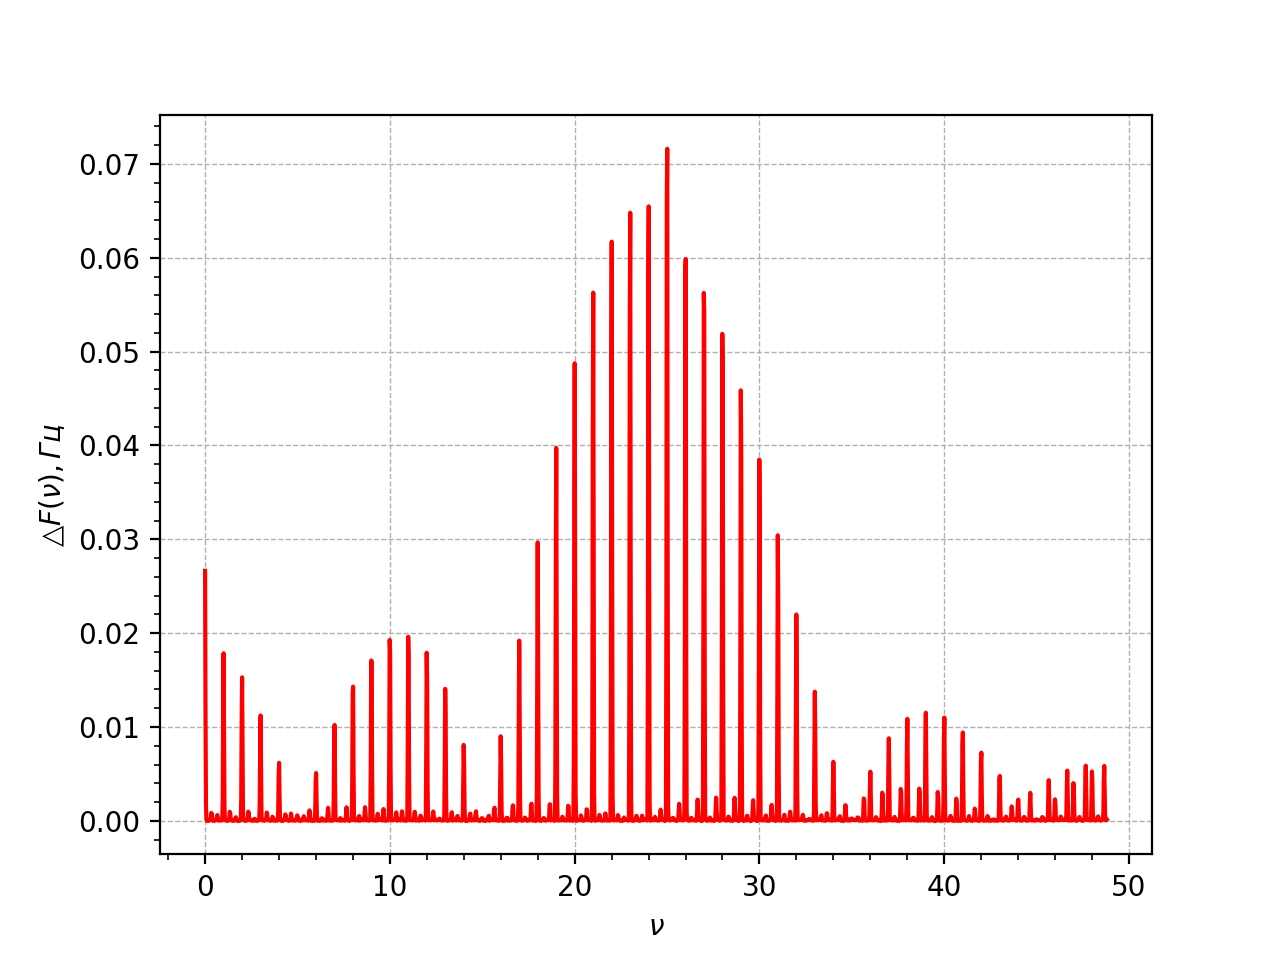
\includegraphics[width=\linewidth]{4.png}\\
\begin{center}
"Эталонный спектр"
\end{center}
\end{minipage}
\begin{minipage}{0.1\textwidth}
\ \ \ \ \ \ \Rightarrow
\end{minipage}
\begin{minipage}{0.44\textwidth}
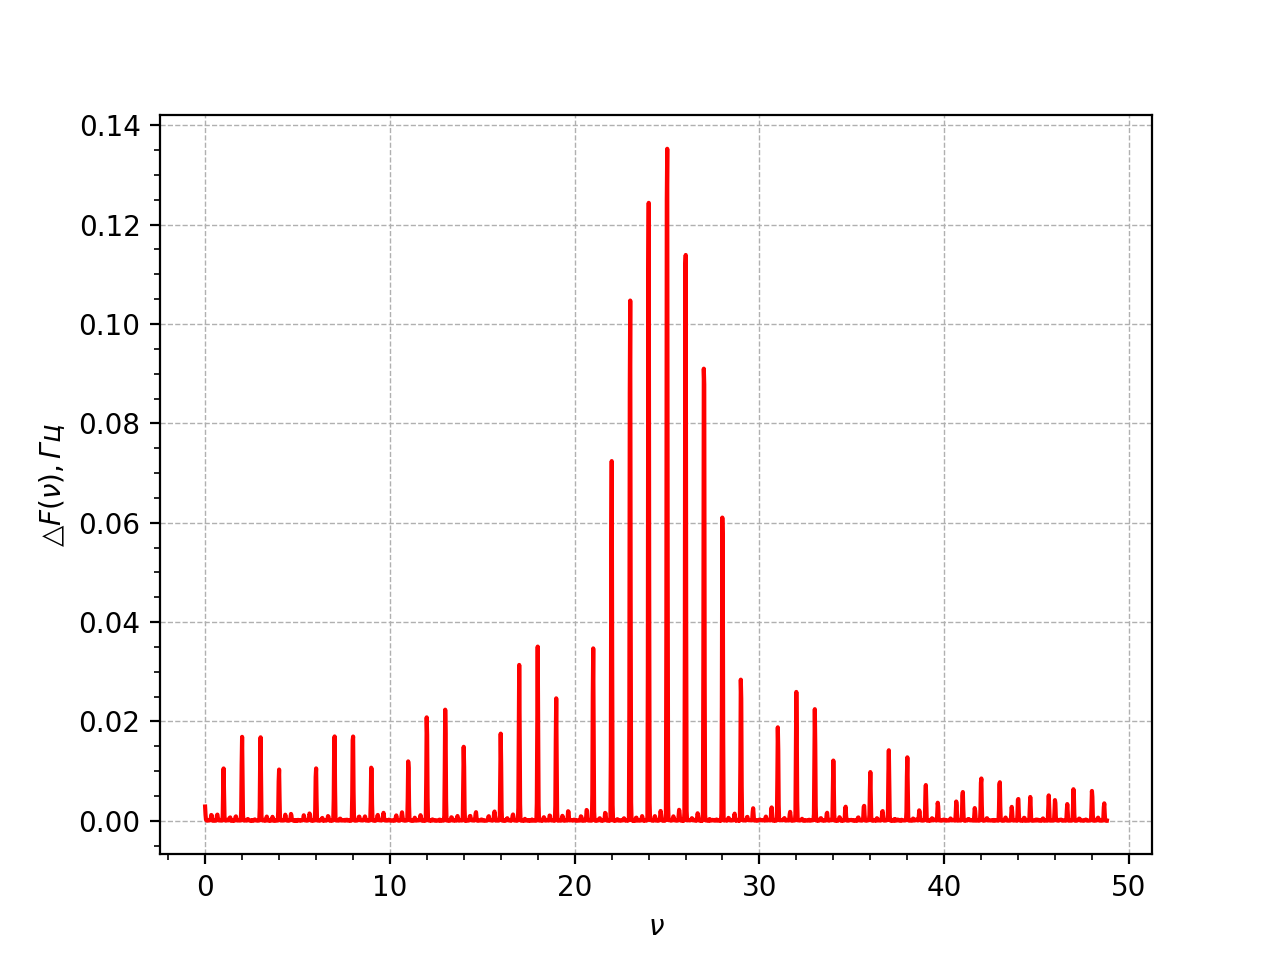
\includegraphics[width=\linewidth]{5.png}\\
\begin{center}
"Увеличение $\tau$ вдвое"
\end{center}
\end{minipage}

\\
\
\\
\newpage

б) при изменении частоты несущей: $\nu_{0}=25,10$ или 40 кГц. изменяется только положение пика. \\

\begin{minipage}{0.3\textwidth}
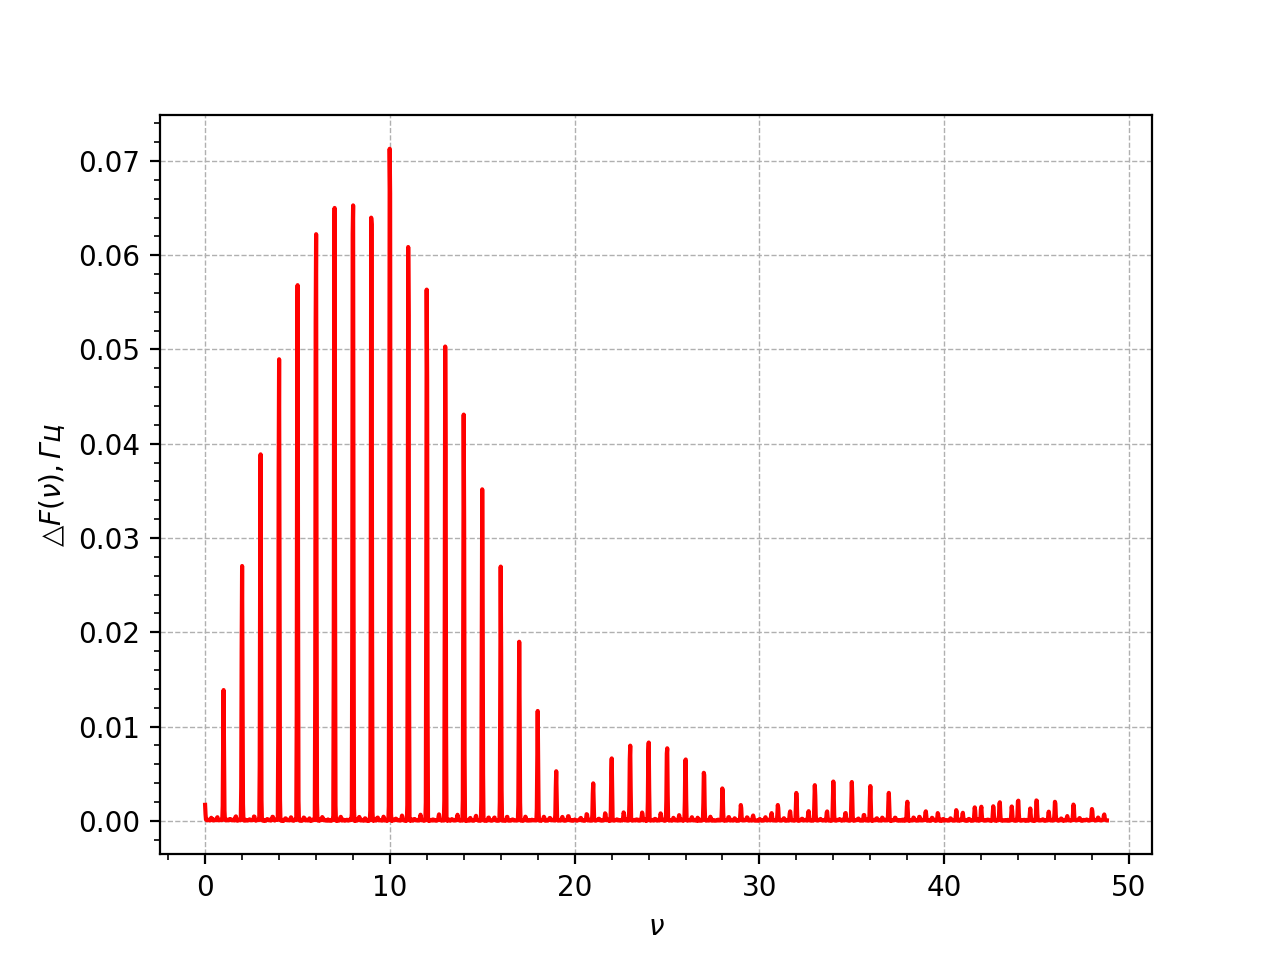
\includegraphics[width=\linewidth]{6.png}\\
\begin{center}
\ \ \ \ \ \ \ \ \ \ \ \ \nu_{0}=10 \ кГц
\end{center}
\end{minipage}
\begin{minipage}{0.05\textwidth}
\begin{center}
\ \ \Rightarrow
\end{center}
\end{minipage}
\begin{minipage}{0.3\textwidth}
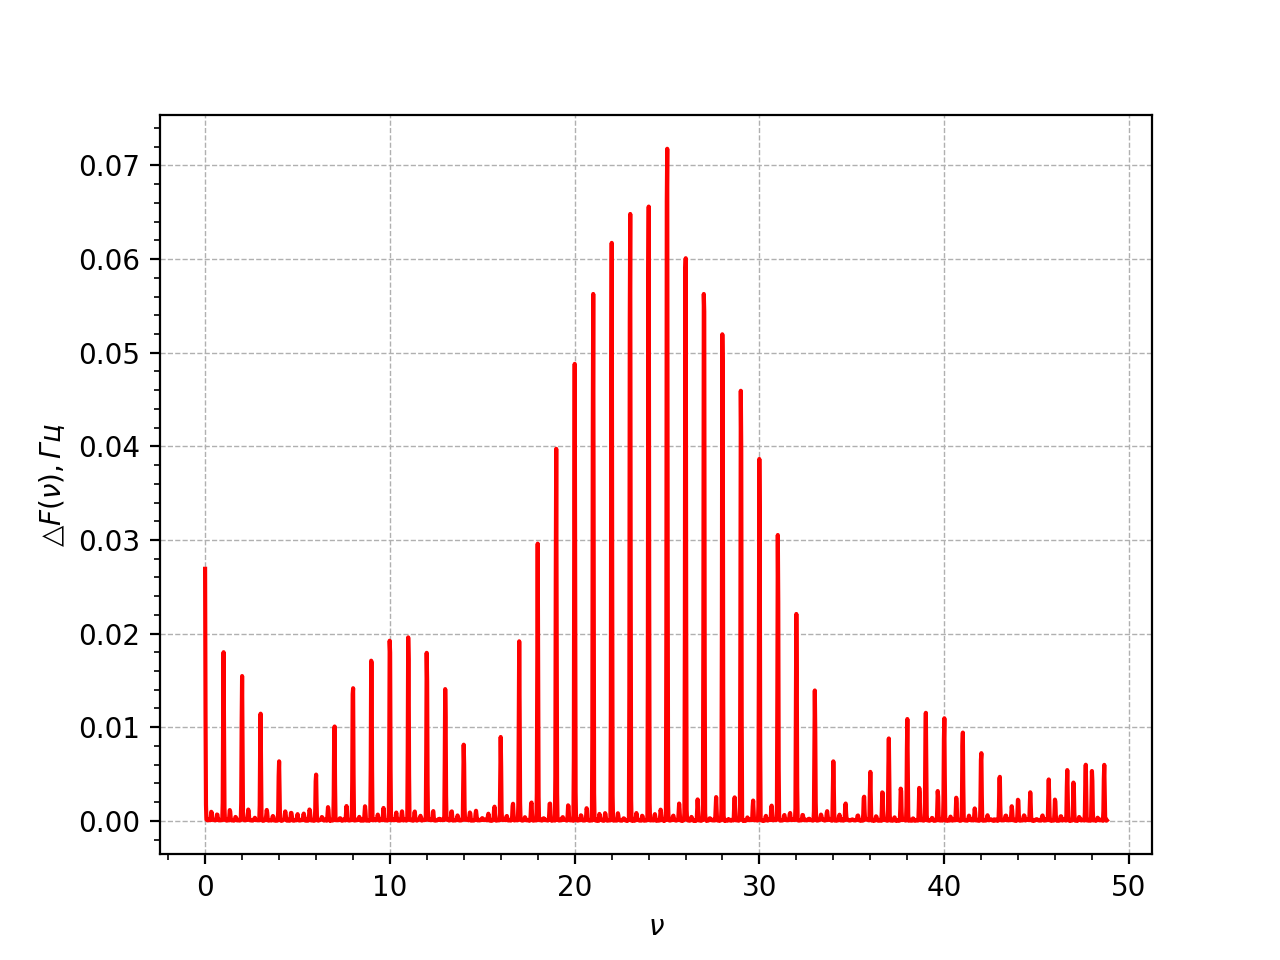
\includegraphics[width=\linewidth]{7.png}\\
\begin{center}
\ \ \ \ \ \ \ \ \ \ \ \ \nu_{0}=25 \ кГц
\end{center}
\end{minipage}
\begin{minipage}{0.05\textwidth}
\begin{center}
\ \ \Rightarrow
\end{center}
\end{minipage}
\begin{minipage}{0.3\textwidth}
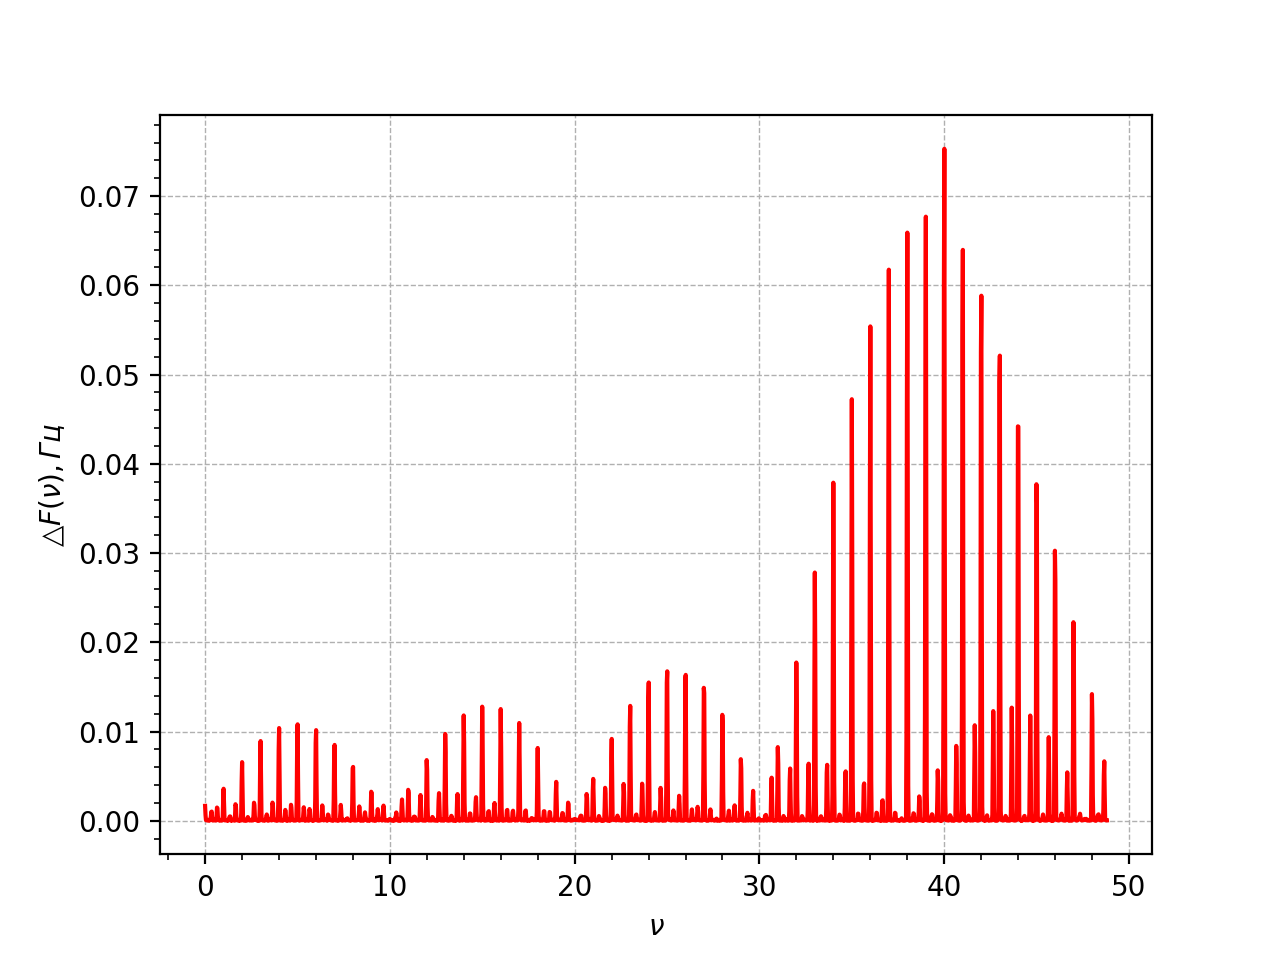
\includegraphics[width=\linewidth]{8.png}\\
\begin{center}
\ \ \ \ \ \ \ \ \ \ \ \ \nu_{0}=40 \ кГц
\end{center}
\end{minipage}


\\
\
\\
\

При фиксированной длительности импульсов $\tau=50$ мкс исследуем зависимость расстояния $\delta \nu$ между соседними спектральными компонентами от периода $T$ (частоты повторения импульсов $f_{\text {повт }}$ В диапазоне $0,5-5 кГц$

\begin{minipage}{0.15\textwidth}
\begin{tabular}{|c|c|c|}
		\hline
		\delta \nu   & f_{\text {повт }}, кГц \\ 
		\hline
0,5   & 0,5\\ 
		\hline
1     &1 \\ 
		\hline
2     &  2 \\ 
		\hline
4     &  4\\ 
		\hline
 5     & 5 \\ 
		\hline
	\end{tabular}
\end{minipage}
\begin{minipage}{0.04\textwidth}
\
\end{minipage}
\begin{minipage}{0.8\textwidth}

\begin{center}
		\begin{tikzpicture}[scale = 1.0]
		\begin{axis}[
		axis lines = left,
		ylabel = {$\delta \nu$},
		xlabel = {$f_{\text {повт }}, кГц$},
		minor grid style={black, line width=0.05pt},
		major grid style={solid,black, line width=0.3pt},
		xmin=0, xmax=5.5,
		ymin=0, ymax=5.5,
		ymajorgrids = true,
		xmajorgrids = true,
		yminorgrids = true,
		xminorgrids = true,
		minor tick num = 4
		]
		\addplot+[only marks ] plot[error bars/.cd, y dir=both, y explicit]
		coordinates {
			(0.5,0.5)
			(1,1)
			(2,2)
			(4,4)
			(5,5)
		};

		\addplot[blue, domain=0:30]{x};
		\end{axis}

		\end{tikzpicture}
		
\end{center}
\begin{center}
\ \ \ \ \ \ \ \ \ \ \  График зависимости $\delta \nu(f_{\text {повт }})$
\end{center}
\end{minipage}

\\

\

По наклону графика можно убедиться в справедливости соотношения неопределённости.

\newpage
Сравним спектры цугов и прямоугольных импульсов при одинаковых значениях $\tau$ и $T$:


\begin{minipage}{0.45\textwidth}
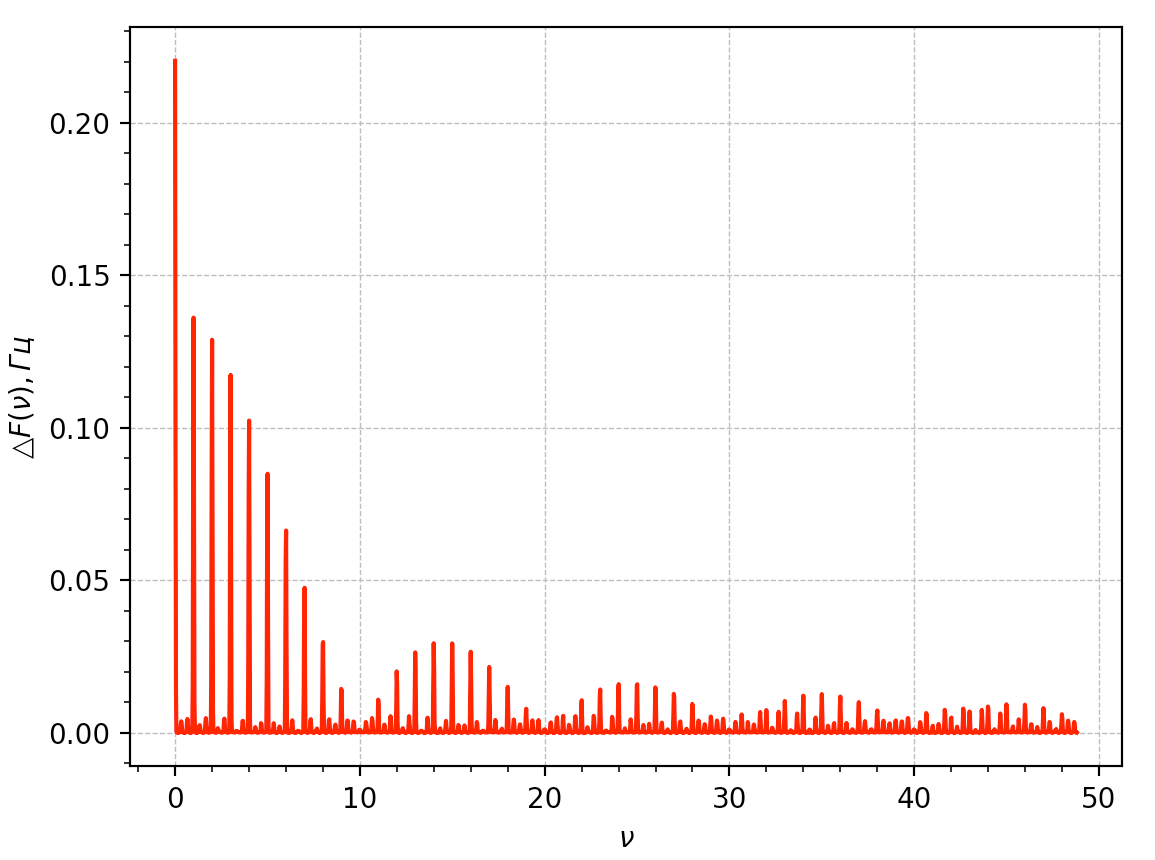
\includegraphics[width=\linewidth]{1.png}\\
\begin{center}
Спектр цугов при $\tau = 100 \ мкс $ и $T = 10^{-3} \ c$
\end{center}
\end{minipage}
\begin{minipage}{0.05\textwidth}
\
\end{minipage}
\begin{minipage}{0.45\textwidth}
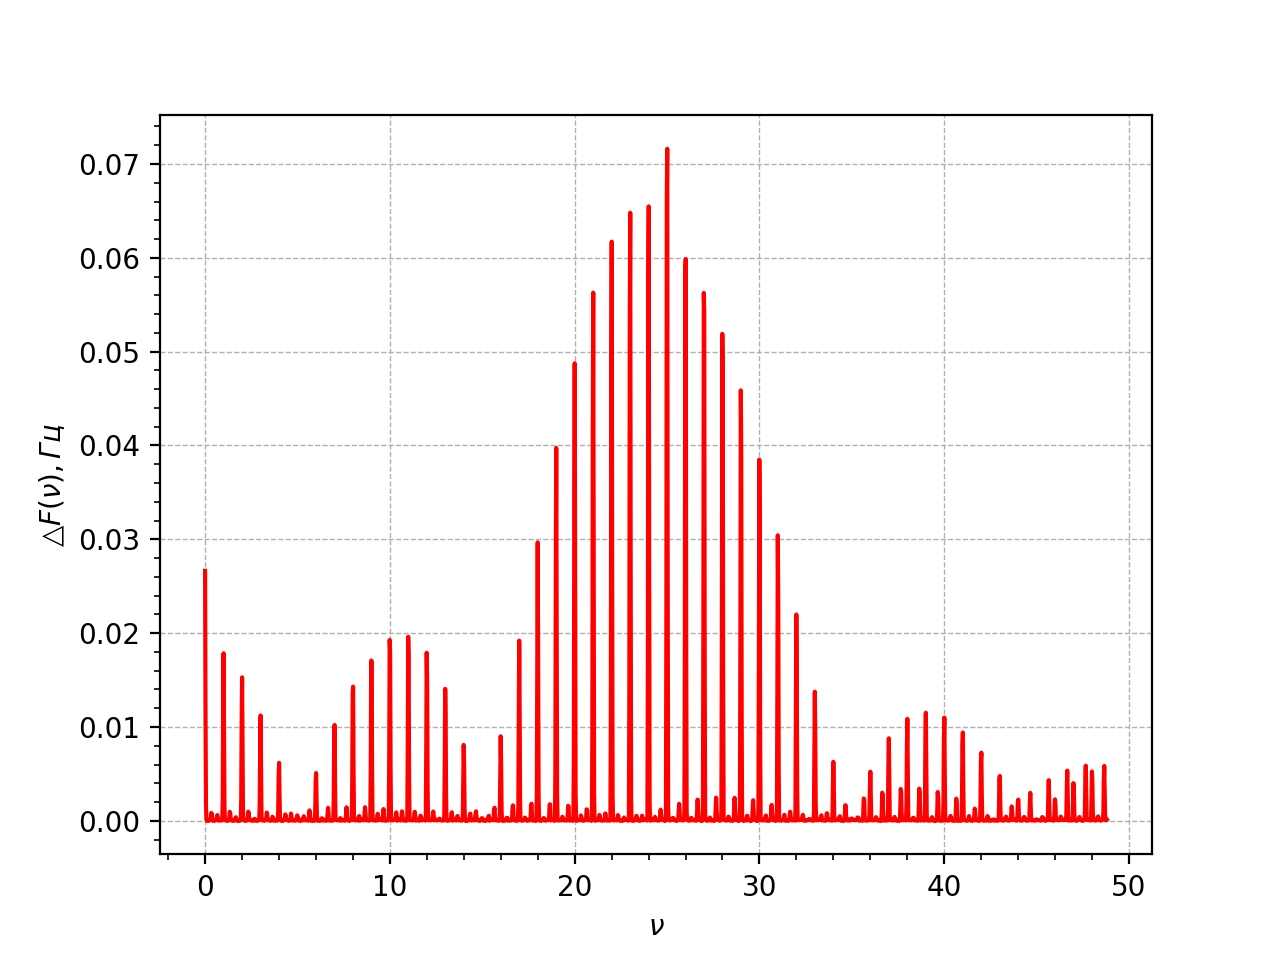
\includegraphics[width=\linewidth]{4.png}\\
\begin{center}
Спектр прямоугольных импульсов при $\tau = 100 \ мкс $ и $T = 10^{-3} \ c$
\end{center}
\end{minipage}


\\
\
\\
\

Явные отличия -- положение пиков и величина амплитуды. 

\subsection{Часть В}

В этой части исследуется зависимость отношения амплитуд спектральных линий синусоидального сигнала, модулированного низкочастотными гармоническими колебаниями, от коэффициента модуляции, который определяется с помощью осциллографа.

Изменяя глубину модуляции, исследуем зависимость отношения амплитуды боковой линии спектра к амплитуде основной линии $\left(a_{\text {бок }} / a_{\text {осн }}\right)$ от глубины модуляции $m ;$ для расчёта глубины модуляции $m$ измерим максимальную $2 A_{\max }$ и минимальную $2 A_{\min }$ амплитуды сигнала на экране осциллографа (см. рис. 6.6 и 6.7). 

\\
\
\\
\

\begin{minipage}{0.45\textwidth}
\begin{tabular}{|c|c|c|c|c|}
		\hline
	A_{max}, В \cdot 10   &A_{min}, В \cdot 10 & A, В & m \\ 
		\hline
   5,55     &  4,50    &   0,2    &     0,104   \\ 
		\hline
   6,02     &   4,02   &     0,4  &   0,199     \\ 
		\hline
	6,59	        &  3,49    & 0,6      &    0,307    \\ 
		\hline
		7,16        & 2,94     &  0,8     &   0,417     \\ 
		\hline
7,56		        &    2,55  &    1,0  &   0,495     \\ 
		\hline
	8,06	        &   2,02   &     1,2  &    0,599    \\ 
		\hline
	8,64	        &    1,49  &    1,4   &    0,705    \\ 
		\hline
	9,16	        &     0,98 &    1,6   &     0,806   \\ 
		\hline
	9,91	        &   0,56   &     1,8  &     0,893   \\ 
		\hline
	1,00	        &    0,17  &    2,0   &    0,966    \\ 
		\hline
	\end{tabular}
\end{minipage}
\begin{minipage}{0.04\textwidth}
\
\end{minipage}
\begin{minipage}{0.45\textwidth}

\begin{center}
		\begin{tikzpicture}[scale = 1.0]
		\begin{axis}[
		axis lines = left,
		ylabel = {$m$},
		xlabel = {$A,\ B$},
		minor grid style={black, line width=0.05pt},
		major grid style={solid,black, line width=0.3pt},
		xmin=0, xmax=2.1,
		ymin=0, ymax=1.05,
		ymajorgrids = true,
		xmajorgrids = true,
		yminorgrids = true,
		xminorgrids = true,
		minor tick num = 4
		]
		\addplot+[only marks ] plot[error bars/.cd, y dir=both, y explicit]
		coordinates {
			(0.2,0.104)
			(0.4,0.199)
			(0.6,0.307)
			(0.8,0.417)
			(1,0.495)
			(1.2,0.599)
			(1.4,0.705)
			(1.6,0.806)
			(1.8,0.893)
			(2,0.966)
		};

		\addplot[blue, domain=0:30]{0.5*x};
		\end{axis}

		\end{tikzpicture}
		
\end{center}
\begin{center}
\ \ \ \ \ \ \ \ \ \ \  Зависимость $m \ от\ A$
\end{center}
\end{minipage}

\\
\
\\
\newpage

Исследуем, как зависит отношнние $a_{\text {бок }} / a_{\mathrm{ocн}}$ от $m$. A_{осн} = 0.323 В. 

\\
\
\\
\

\begin{minipage}{0.45\textwidth}
\begin{tabular}{|c|c|c|c|c|}
		\hline
	A_{бок}, В \cdot 10   &A_{бок}/A_{осн} & A, В & m \\ 
		\hline
   0,016     &  0,048    &   0,2    &     0,104   \\ 
		\hline
   0,032     &   0,097   &     0,4  &   0,199     \\ 
		\hline
	0,048	        &  0,149    & 0,6      &    0,307    \\ 
		\hline
		0,064        & 0,197     &  0,8     &   0,417     \\ 
		\hline
0,078		        &   0,246  &    1,0  &   0,495     \\ 
		\hline
	0,094	        &   0,289   &     1,2  &    0,599    \\ 
		\hline
	0,110	        &    0,341  &    1,4   &    0,705    \\ 
		\hline
	0,128	        &     0,396 &    1,6   &     0,806   \\ 
		\hline
	0,142	        &   0,440   &     1,8  &     0,893   \\ 
		\hline
	0,162	        &    0,500  &    2,0   &    0,966    \\ 
		\hline
	\end{tabular}
\end{minipage}
\begin{minipage}{0.04\textwidth}
\
\end{minipage}
\begin{minipage}{0.45\textwidth}

\begin{center}
		\begin{tikzpicture}[scale = 1.0]
		\begin{axis}[
		axis lines = left,
		ylabel = {$m$},
		xlabel = {$A_{бок}/A_{осн}$},
		minor grid style={black, line width=0.05pt},
		major grid style={solid,black, line width=0.3pt},
		xmin=0, xmax=0.55,
		ymin=0, ymax=1.05,
		ymajorgrids = true,
		xmajorgrids = true,
		yminorgrids = true,
		xminorgrids = true,
		minor tick num = 4
		]
		\addplot+[only marks ] plot[error bars/.cd, y dir=both, y explicit]
		coordinates {
			(0.048,0.104)
			(0.097,0.199)
			(0.149,0.307)
			(0.197,0.417)
			(0.246,0.495)
			(0.289,0.599)
			(0.341,0.705)
			(0.396,0.806)
			(0.440,0.893)
			(0.5,0.966)
		};

		\addplot[blue, domain=0:30]{2*x};
		\end{axis}

		\end{tikzpicture}
		
\end{center}
\begin{center}
\ \ \ \ \ \ \ \ \ \ \  Зависимость $m \ от\ A_{бок}/A_{осн}$
\end{center}
\end{minipage}

\\
\
\\


 Угол наклона графика равен 2. 

\section{Выводы}

Исследования зависимости ширины спектра периодической последовательности прямоугольных импульсов от длительности отдельного импульса в первой части работы полностью совпали с теоретическими рассчетами. По наклону графика из этой части можно убедиться в соотношении неопределенностей ($\quad \Delta \nu \Delta t \simeq 1$).
 
Исследования зависимости расстояния между ближайшими спектральными компонентами от частоты повторения цугов дали схожие резкльтаты. 

В последней части коэффициенты, получаемые в результате исследования зависимости отношения амплитуд спектральных линий синусоидального сигнала, модулированного низкочастотными гармоническими колебаниями, от коэффициента модуляции полностью совпали с теоретически рассчитаными. 


\end{document}
